\section{Experiments}
\label{sec:experiments}

In this section we describe experiments based on our testing framework. 

%%%%%

\begin{figure}
\begin{center}
\begin{tabular}{lccc}
Category            & Arity & Stateful? & Heterogeneous? \\ \hline
Synchronous channel & 2     & N         & Y \\
Filter channel      & 2     & N         & Y \\
Men and women        & 2     & N         & Y \\
Exchanger           & 2     & N         & N \\
Two families        & 2     & Y         & Y \\
One family          & 2     & Y         & N \\
ABC                 & 3     & N         & Y \\
Barrier             & $n$   & N         & N \\
Enrollable barrier  & $1\mathord{..} n$, 1 & Y & N \\
Timeout channel     & 2, 1  & N         & Y \\
Timeout exchanger   & 2, 1  & N         & N \\
Closeable channel   & 2, 1  & Y         & Y \\
Terminating queue   & 1, $n$ & Y        & N  
\end{tabular}
\end{center}
\caption{Example interfaces of synchronisation objects.  \label{fig:examples}}
\end{figure}

% Channel with counter & 2    & Y         & Y \\
% ABC with counter    & 3     & Y         & Y \\
% Barrier with counter & $n$  & Y         & N \\   
% Add combining barrier?    

%%%%%

We consider synchronisation objects implementing a number of interfaces,
summarised in Figure~\ref{fig:examples}.  Most of the interfaces were
described in earlier sections (namely synchronous channel, filter channel,
exchanger, barrier, timeout channel, closable channel, enrollable barrier, and
terminating queue).
%
The \emph{men and women} problem involves two families of threads, known as
men and women: each thread wants to pair off with a thread of the other type;
each passes in its own identity, and expects to receive back the identity of
the thread with which it has paired.  
%
In the \emph{two families} problem,
there are two families of threads, with $n$~threads of each family; each
thread calls an operation~$n$ times, and each invocation should synchronise
with a thread of the opposite family, a different thread each time.  In the
\emph{one family} problem, there are $n$~threads, each of which calls an
operation $n-1$~times, and each time should synchronise with a different
thread.  
%
The \emph{ABC} problem can be thought of as a ternary version of the men and
women problem: there are three types of threads, A, B and C; each
synchronisation involves one thread of each type.  
%
%% The \emph{enrollable barrier} (based on ~\cite{alting-barrier}) is a barrier
%% that allows threads to enrol and resign (via unary operations); each barrier
%% synchronisation is between all threads that are currently enrolled; thus the
%% barrier has a state, namely the currently enrolled threads. 
%
Finally, the \emph{timeout exchanger} is a timed version of the exchanger: if
a thread fails to exchange data with another thread, it can timeout and return
an appropriate result.

%% For each interface, we have implemented a tester, using the appropriate
%% algorithm from earlier sections.  When considering synchronisation
%% linearisation, in most cases, the invocations performed by threads had to be
%% chosen so that every invocation will synchronise, so as to avoid deadlocks.
%% For example, for the synchronous channel tester, half the threads perform
%% sends, and half perform receives; in the exchanger tester, each thread ran a
%% single invocation (or else a slow thread could get stuck).

%% For synchronisation objects involving data, the data values were chosen
%% randomly from a reasonably large range (e.g.~$\range{0}{100}$); this makes it
%% easier for the algorithm to identify matchings, and also makes it easier for
%% the user to understand any incorrect histories that are detected.  The
%% implementations are data independent~\cite{???}: they store and return the
%% data, but otherwise their operation does not depend on the data values used;
%% this means that the data values used do not affect the occurrences of bugs.

For each interface, we have implemented testers, using both the two-step
approach from Section~\ref{sec:lin-testing}, and the direct algorithm from
Section~\ref{sec:direct}.

For each interface, we have produced a correct implementation.  For most
interfaces, we have also implemented one or more faulty versions that fail to
achieve either synchronisation linearisation or progressibility.  The faulty
versions mostly have realistic mistakes: mistakes that we believe programmers
could make.

%%%%%%%%%%%%%%%%%%%%%%%%%%%%%%%%%%%%%%%%%%%%%%%%%%%%%%%

\subsection{Experiments}


We describe various experiments below.  Questions we want to answer include:
\begin{itemize}
\item Which works better, the direct algorithm or the two-step algorithm?  
\item How should we choose parameters (number of threads to run, number of
  iterations performed by each thread, etc.)\ for testing?  
\item Is this approach effective at finding bugs?
\end{itemize}
%
The purpose of testing is to find bugs.  We therefore concentrate on the time
taken to find bugs.


The experiments were performed on a dedicated eight-core machine (two 2.40GHz
Intel(R) Xeon(R) E5620 CPUs, with 12GB of RAM, but limited to 4GB of heap
space).

In each experiment below, we performed a number of \emph{runs} of a tester on
a synchronisation object with a bug that causes a failure
of synchronisation linearisation, but does not lead to a deadlock.  In each
run, a particular number of threads performed a particular number of operation
calls on the synchronisation object; the relevant algorithm was then used to
decide whether the log history was synchronisation linearisable or two-step
linearisable.

Each \emph{observation} performed multiple runs until an error was detected.
Each observation was performed as a separate operating system process, with
the aim of making observations independent, avoiding dependencies caused by,
for example garbage collection, caching behaviour, and just-in-time
compilation.  Thus each observation was as close as possible to a normal use
case.

For each data point in the experiments, we performed multiple observations.
We give the average running time and a 95\%-confidence interval.  The number
of observations is chosen so as to obtain a reasonably small confidential
interval, but avoiding excessively long experiments.

%%%%%%%%%%%%%%%%%%%%%%%%%%%%%%%%%%%%%%%%%%%%%%%%%%%%%%%

We start with the second of the questions above, how to choose parameters for
testing.  Each of the graphs in Figures~\ref{fig:params-experiment-1}
and~\ref{fig:params-experiment-2} concerns a particular
tester.  Each data point represents a particular number of threads (given in
the key), and a particular number of operation executions by each thread
(given on the $X$-axis), with 100 observations.  The $Y$-axis gives the time
in milliseconds. 


%% \documentclass[a4paper]{article}
%% \usepackage{pgfplots}
%% \pgfplotsset{compat=1.16}
%% \begin{document}


%\pgfplotsset{every semilogxaxis/.append style = { cycle list name=my mark list, }}

\def\gHeight{0.4579\textheight}
\def\gWidth{0.50\textwidth}
%% With labels on axes
%% \def\gHeight{0.44\textheight}
%% \def\gWidth{0.35\textwidth}

\begin{figure}
\begin{center}
\begin{tikzpicture}
\begin{semilogxaxis}[
  title = {Synchronous channel, direct},
 % Experiment on the time taken to find a bug using ChanTester --faulty,
  %% ylabel = Time (ms),
  %% xlabel = Number of iterations per thread,
  ymin = 0,
  log basis x=2,
  scaled ticks = false,
  legend pos = south east,
  height = \gHeight,
  width = \gWidth,
  cycle list name=my mark list,
]
\addplot+[error bars/.cd, y dir=both,y explicit] coordinates {
  (2,86.12661781999999) +- (0,1.7917221449438974)
  (4,80.95611876999999) +- (0,2.151870544775658)
  (8,79.33566509) +- (0,2.2847148738449485)
  (16,75.60885972) +- (0,2.077410210931587)
  (32,75.91483873) +- (0,1.77206458988127)
};
\addlegendentry{$p$ = 2}
\addplot+[error bars/.cd, y dir=both,y explicit] coordinates {
  (2,88.15634318000001) +- (0,2.280526062395564)
  (4,82.28905311) +- (0,2.3893457135505605)
  (8,81.42642638) +- (0,2.343502687069828)
  (16,81.70105392) +- (0,2.19568045053051)
  (32,83.99210701000001) +- (0,1.1896791019624882)
};
\addlegendentry{$p$ = 4}
\addplot+[error bars/.cd, y dir=both,y explicit] coordinates {
  (2,88.53399624) +- (0,2.5770165231292586)
  (4,86.50421789) +- (0,1.8202756998260026)
  (8,88.31893217) +- (0,1.0446761315476831)
  (16,92.69791773) +- (0,1.1625119157788526)
  (32,100.82756555) +- (0,1.026210111624912)
};
\addlegendentry{$p$ = 8}
\addplot+[error bars/.cd, y dir=both,y explicit] coordinates {
  (2,100.60871656) +- (0,3.421021184767031)
  (4,98.96857434) +- (0,1.5976825567761581)
  (8,102.43561928) +- (0,1.0967809472697325)
  (16,111.79526836) +- (0,1.331421208545199)
};
\addlegendentry{$p$ = 16}
\end{semilogxaxis}
\end{tikzpicture}
%%%%%%%%%%%
\hfill%
\begin{tikzpicture}
\begin{semilogxaxis}[
  title = {Synchronous channel, two-step},
% Experiment on the time taken to find a bug using ChanTwoStepTester --faulty,
  %% ylabel = Time (ms),
  %% xlabel = Number of iterations per thread,
  ymin = 0,
  log basis x=2,
  scaled ticks = false,
  legend pos = south east,
  height = \gHeight,
  width = \gWidth,
  cycle list name=my mark list,
]
\addplot+[error bars/.cd, y dir=both,y explicit] coordinates {
  (2,97.48732987000001) +- (0,2.537052448574137)
  (4,98.00178478) +- (0,0.7155620511380979)
  (8,102.59852943000001) +- (0,1.248428236383366)
  (16,110.18692125) +- (0,1.8779254833338999)
  (32,122.86119026) +- (0,3.687510258368647)
};
\addlegendentry{$p$ = 2}
\addplot+[error bars/.cd, y dir=both,y explicit] coordinates {
  (2,103.68578293) +- (0,0.9185773564133626)
  (4,107.72147869) +- (0,1.1262832580516602)
  (8,115.23526969) +- (0,1.558869648950144)
  (16,129.42642214) +- (0,2.890432405032626)
  (32,147.61696638) +- (0,3.3701479571174087)
};
\addlegendentry{$p$ = 4}
\addplot+[error bars/.cd, y dir=both,y explicit] coordinates {
  (2,115.59173774) +- (0,1.1624918696707782)
  (4,129.18186215) +- (0,3.0346089254020145)
  (8,149.27067307) +- (0,4.752304398606616)
  (16,184.42443716) +- (0,8.787981873362584)
  (32,224.80307553999998) +- (0,12.904969334685587)
};
\addlegendentry{$p$ = 8}
\end{semilogxaxis}
\end{tikzpicture}

%%%%%%%%%%%%%%%%%%%%%%%%%%%%%%%%%%%%%%%%%%%%%%%%%%%%%%%

\begin{tikzpicture}
\begin{semilogxaxis}[
  title = {ABC problem, direct},
% Experiment on the time taken to find a bug using ABCTester --faulty,
  %% ylabel = Time (ms),
  %% xlabel = Number of iterations per thread,
  ymin = 0, ymax = 12000,
  log basis x=2,
  scaled ticks = false,
  legend pos = north east,
  height = \gHeight,
  width = \gWidth,
  cycle list name=my mark list,
]
\addplot+[error bars/.cd, y dir=both,y explicit] coordinates {
  (2,63148.00490261) +- (0,21759.613507248898)
  (4,651.16099215) +- (0,172.9165504857434)
  (8,889.50264446) +- (0,253.67598564893999)
  (16,988.93800777) +- (0,331.2238136254922)
  (32,2531.2923463800003) +- (0,637.8365814648288)
};
\addlegendentry{$p$ = 6}
\addplot+[error bars/.cd, y dir=both,y explicit] coordinates {
  (2,8285.14449145) +- (0,2778.240180885241)
  (4,538.35292637) +- (0,69.7619752736345)
  (8,570.41879925) +- (0,72.51216157132927)
  (16,1236.46460153) +- (0,603.1643293373226)
};
\addlegendentry{$p$ = 9}
\addplot+[error bars/.cd, y dir=both,y explicit] coordinates {
  (2,2353.5410284299996) +- (0,556.6201735112219)
  (4,425.88017894) +- (0,43.38091364960696)
  (8,460.78079447000005) +- (0,55.267882094272984)
  (16,927.89629072) +- (0,310.78678210463266)
};
\addlegendentry{$p$ = 15}
\addplot+[error bars/.cd, y dir=both,y explicit] coordinates {
  (2,2086.92048954) +- (0,486.9798287963568)
  (4,457.24736308999996) +- (0,57.960262260725735)
  (8,815.22070533) +- (0,137.83521886164093)
};
\addlegendentry{$p$ = 24}
\end{semilogxaxis}
\end{tikzpicture}
%%%%%%
\hfill%
\begin{tikzpicture}
\begin{semilogxaxis}[
  title = {ABC problem, two-step},
% Experiment on the time taken to find a bug using ABCTwoStepTester --faulty,
  %% ylabel = Time (ms),
  %% xlabel = Number of iterations per thread,
  ymin = 0, ymax = 12000,
  log basis x=2,
  scaled ticks = false,
  legend pos = north east,
  height = \gHeight,
  width = \gWidth,
  cycle list name=my mark list,
]
\addplot+[error bars/.cd, y dir=both,y explicit] coordinates {
  (2,65758.65076251) +- (0,25549.72875338341)
  (4,1045.58266548) +- (0,329.4516890468716)
  (8,1046.70000612) +- (0,190.21621707113712)
  (16,2034.9508281300002) +- (0,663.4683619888534)
};
\addlegendentry{$p$ = 6}
\addplot+[error bars/.cd, y dir=both,y explicit] coordinates {
  (2,8272.18414539) +- (0,2218.9195185871336)
  (4,647.6533947300001) +- (0,91.52294872037436)
  (8,877.6609487100001) +- (0,115.20504848610265)
};
\addlegendentry{$p$ = 9}
\addplot+[error bars/.cd, y dir=both,y explicit] coordinates {
  (2,3214.8299765799998) +- (0,832.8638371203842)
  (4,614.13599756) +- (0,80.38135215280637)
  (8,1010.49079758) +- (0,131.23949278860303)
};
\addlegendentry{$p$ = 12}
\end{semilogxaxis}
\end{tikzpicture}
\end{center}
\caption{Effect of choices of parameters for testers for a synchronous channel
  and the ABC problem.}
\label{fig:params-experiment-1}
\end{figure}

%%%%%%%%%%%%%%%%%%%%%%%%%%%%%%%%%%%%%%%%%%%%%%%%%%%%%%%
%%%%%%%%%%%%%%%%%%%%%%%%%%%%%%%%%%%%%%%%%%%%%%%%%%%%%%%

\begin{figure}
\begin{center}
\begin{tikzpicture}
\begin{semilogxaxis}[
  title = {Barrier, direct},
% Experiment on the time taken to find a bug using BarrierTester --faulty4,
  %% ylabel = Time (ms),
  %% xlabel = Number of iterations per thread,
  ymin = 0,
  log basis x=2,
  scaled ticks = false,
  legend pos = south east,
  height = \gHeight,
  width = \gWidth,
  cycle list name=my mark list,
]
\addplot+[error bars/.cd, y dir=both,y explicit] coordinates {
  (2,79.78356759) +- (0,0.6753803761895055)
  (4,80.21149943) +- (0,0.7417077841043016)
  (8,82.15990262999999) +- (0,0.9721482587110002)
  (16,85.56849578) +- (0,1.3170026624624744)
  (32,89.00165894) +- (0,1.214991840184841)
};
\addlegendentry{$p$ = 2}
\addplot+[error bars/.cd, y dir=both,y explicit] coordinates {
  (2,80.69491434) +- (0,1.277121828349371)
  (4,79.11638876) +- (0,0.8541881324957225)
  (8,82.34575759) +- (0,0.6647658092993566)
  (16,90.96288109999999) +- (0,0.7946518374359616)
  (32,105.6103622) +- (0,0.9084773991480668)
};
\addlegendentry{$p$ = 4}
\addplot+[error bars/.cd, y dir=both,y explicit] coordinates {
  (2,87.37795215000001) +- (0,1.148427979634296)
  (4,91.80450587) +- (0,0.9659897545948385)
  (8,101.90022009) +- (0,1.0396303105810654)
  (16,114.59724041) +- (0,1.2234727441382758)
  (32,134.96979653) +- (0,1.3399123540734243)
};
\addlegendentry{$p$ = 8}
\addplot+[error bars/.cd, y dir=both,y explicit] coordinates {
  (2,103.75736121) +- (0,1.1028844359069854)
  (4,114.74564184) +- (0,1.065963299194866)
  (8,126.3824616) +- (0,1.2558203057125663)
  (16,146.69931995) +- (0,1.4325749994158248)
};
\addlegendentry{$p$ = 16}
\end{semilogxaxis}
\end{tikzpicture}
%%%%%
\hfill%
\begin{tikzpicture}
\begin{semilogxaxis}[
  title = {Barrier, two-step},
% Experiment on the time taken to find a bug using BarrierTwoStepTester --faulty4,
  %% ylabel = Time (ms),
  %% xlabel = Number of iterations per thread,
  ymin = 0,
  log basis x=2,
  scaled ticks = false,
  legend style={at={(0.95,0.5)}},
  %legend pos = south east,
  height = \gHeight,
  width = \gWidth,
  cycle list name=my mark list,
]
\addplot+[error bars/.cd, y dir=both,y explicit] coordinates {
  (2,104.52545672) +- (0,1.1384114955505373)
  (4,106.5277703) +- (0,0.8659686125977645)
  (8,110.02191739) +- (0,1.0478095390846915)
  (16,117.76376726000001) +- (0,1.4735785997288966)
  (32,126.09393337) +- (0,1.2584474029641417)
};
\addlegendentry{$p$ = 4}
\addplot+[error bars/.cd, y dir=both,y explicit] coordinates {
  (2,473.48318351) +- (0,6.665762120027659)
  (4,484.3246579) +- (0,7.588975675101476)
  (8,491.51942674000003) +- (0,5.436439641721073)
  (16,499.12677864999995) +- (0,6.026954379109569)
  (32,507.43132356) +- (0,7.060360684052092)
};
\addlegendentry{$p$ = 8}
\addplot+[error bars/.cd, y dir=both,y explicit] coordinates {
  (2,4723.944651850001) +- (0,88.7333271725884)
  (4,5140.44886425) +- (0,390.9244260810367)
  (8,4984.51105782) +- (0,299.05582122501505)
  (16,4846.063625010001) +- (0,185.3313893605648)
};
\addlegendentry{$p$ = 10}
\end{semilogxaxis}
\end{tikzpicture}

%%%%%%%%%%%%%%%%%%%%%%%%%%%%%%%%%%%%%%%%%%%%%%%%%%%%%%%

%% \begin{tikzpicture}
%% \begin{semilogxaxis}[
%%   title = {Exchanger, direct},
%% % Experiment on the time taken to find a bug using ExchangerTester --faulty,
%%   %% ylabel = Time (ms),
%%   %% xlabel = Number of iterations per thread,
%%   ymin = 0,
%%   log basis x=2,
%%   scaled ticks = false,
%%   legend pos = south east,
%%   height = \gHeight,
%%   width = \gWidth
%% ]
%% \addplot+[error bars/.cd, y dir=both,y explicit] coordinates {
%%   (2,79.4980078) +- (0,4.969728356062269)
%%   (4,81.5675652) +- (0,5.717326619474392)
%%   (8,77.60383034) +- (0,4.690777171745089)
%%   (16,81.10696336) +- (0,5.719550651715445)
%%   (32,81.79361565) +- (0,5.464883215270754)
%% };
%% \addlegendentry{$p$ = 4}
%% \addplot+[error bars/.cd, y dir=both,y explicit] coordinates {
%%   (2,73.68581234999999) +- (0,1.1772616810952101)
%%   (4,74.12068856) +- (0,2.2298505104315494)
%%   (8,74.53505454) +- (0,2.12662706415007)
%%   (16,74.04116777) +- (0,1.173710689795218)
%%   (32,76.37519547) +- (0,4.468775877914856)
%% };
%% \addlegendentry{$p$ = 8}
%% \addplot+[error bars/.cd, y dir=both,y explicit] coordinates {
%%   (2,83.19619601000001) +- (0,1.0357204067709476)
%%   (4,84.16564632) +- (0,1.0339471730559555)
%%   (8,83.61105594) +- (0,1.1567691820915948)
%%   (16,83.87681695) +- (0,1.1166611666195976)
%%   (32,83.29783656999999) +- (0,0.9106413255446043)
%% };
%% \addlegendentry{$p$ = 16}
%% \addplot+[error bars/.cd, y dir=both,y explicit] coordinates {
%%   (2,112.2743958) +- (0,2.4499531527325344)
%%   (4,112.05081016) +- (0,2.1363049579932554)
%%   (8,110.72104375) +- (0,2.154547825270566)
%%   (16,113.45533171) +- (0,2.3122404291087393)
%% };
%% \addlegendentry{$p$ = 32}
%% \end{semilogxaxis}
%% \end{tikzpicture}
%% %%%%%
%% \hfill%
%% \begin{tikzpicture}
%% \begin{semilogxaxis}[
%%   title = {Exchanger, two-step},
%% % Experiment on the time taken to find a bug using ExchangerTwoStepTester --faulty,
%%   %% ylabel = Time (ms),
%%   %% xlabel = Number of iterations per thread,
%%   ymin = 0,
%%   log basis x=2,
%%   scaled ticks = false,
%%   %legend pos = north east,
%%   legend style={at={(0.95,0.5)}},
%%   height = \gHeight,
%%   width = \gWidth
%% ]
%% \addplot+[error bars/.cd, y dir=both,y explicit] coordinates {
%%   (2,123.86405796) +- (0,8.037523435641969)
%%   (4,116.22122895) +- (0,5.163792850498938)
%%   (8,117.38155825) +- (0,4.1538189226791475)
%%   (16,127.48406541) +- (0,8.069867651568115)
%%   (32,123.89457534) +- (0,5.784136268257348)
%% };
%% \addlegendentry{$p$ = 4}
%% \addplot+[error bars/.cd, y dir=both,y explicit] coordinates {
%%   (2,535.28604669) +- (0,24.91982914948026)
%%   (4,489.79530002999996) +- (0,30.018925715872925)
%%   (8,501.71219262) +- (0,28.351449932028633)
%%   (16,483.71662317) +- (0,29.4417123713682)
%%   (32,482.93430472000006) +- (0,30.11208912390406)
%% };
%% \addlegendentry{$p$ = 8}
%% \addplot+[error bars/.cd, y dir=both,y explicit] coordinates {
%%   (2,4964.56554911) +- (0,522.4975339054702)
%%   (4,4489.6878968500005) +- (0,489.42545179368557)
%%   (8,4783.7948075) +- (0,482.77575329662307)
%%   (16,4696.5925643) +- (0,541.8583452036177)
%%   (32,5075.38201705) +- (0,513.4696344347326)
%% };
%% \addlegendentry{$p$ = 10}
%% \end{semilogxaxis}
%% \end{tikzpicture}
%% \end{center}
%% \caption{Effect of choices of parameters for testers for a barrier and an
%%   exchanger.}
%% \label{fig:params-experiment-2}
%% \end{figure}

%%%%%%%%%%%%%%%%%%%%%%%%%%%%%%%%%%%%%%%%%%%%%%%%%%%%%%%
%%%%%%%%%%%%%%%%%%%%%%%%%%%%%%%%%%%%%%%%%%%%%%%%%%%%%%%

%% \begin{figure}
%% \begin{center}
\begin{tikzpicture}
\begin{semilogxaxis}[
  title = {Closeable channel, direct},
% Experiment on the time taken to find a bug using CloseableChanTester --faultyWrapped,
  %% ylabel = Time (ms),
  %% xlabel = Number of iterations per thread,
  ymin = 0,
  log basis x=2,
  scaled ticks = false,
  legend pos = north east,
  height = \gHeight,
  width = \gWidth,
  cycle list name=my mark list,
]
\addplot+[error bars/.cd, y dir=both,y explicit] coordinates {
  (2,217.87036477) +- (0,20.95342905917427)
  (4,230.86778241) +- (0,19.798701188208636)
  (8,261.64808591999997) +- (0,22.670538051657655)
  (16,260.33807355) +- (0,21.011043536506982)
  (32,283.35029041) +- (0,24.207343654890213)
};
\addlegendentry{$p$ = 2}
\addplot+[error bars/.cd, y dir=both,y explicit] coordinates {
  (2,211.16205488999998) +- (0,11.940481774546184)
  (4,201.49129182) +- (0,11.327761520940962)
  (8,209.65499441) +- (0,11.493818434761115)
  (16,227.03573612) +- (0,13.275939252852606)
  (32,245.23078971) +- (0,12.431403656046855)
};
\addlegendentry{$p$ = 4}
\addplot+[error bars/.cd, y dir=both,y explicit] coordinates {
  (2,229.76947737) +- (0,13.333998715056868)
  (4,205.40328603) +- (0,7.113226630181317)
  (8,215.71346077) +- (0,8.57622815594333)
  (16,225.81513956) +- (0,9.079828437001673)
  (32,269.27598687) +- (0,13.53010438846008)
};
\addlegendentry{$p$ = 8}
\addplot+[error bars/.cd, y dir=both,y explicit] coordinates {
  (2,411.6651253) +- (0,67.13326503788613)
  (4,567.7329529) +- (0,216.01117553300745)
  (8,495.66493997000003) +- (0,104.46284260122805)
  (16,556.55072212) +- (0,134.35063241398308)
};
\addlegendentry{$p$ = 16}
\end{semilogxaxis}
\end{tikzpicture}
%%%%%%%%%%%%%%%%%%%%%%%%%
\hfill%
\begin{tikzpicture}
\begin{semilogxaxis}[
  title = {Closeable channel, two-step},
%Experiment on the time taken to find a bug using CloseableChannelTwoStepTester --faultyWrapped,
  %% ylabel = Time (ms),
  %% xlabel = Number of iterations per thread,
  ymin = 0, ymax = 700,
  log basis x=2,
  scaled ticks = false,
  legend pos = north east,
  height = \gHeight,
  width = \gWidth,
  cycle list name=my mark list,
]
\addplot+[error bars/.cd, y dir=both,y explicit] coordinates {
  (2,219.9772513) +- (0,15.934906768096278)
  (4,209.06976327) +- (0,15.358697413263384)
  (8,214.01946236) +- (0,15.628095370426285)
  (16,261.98785987) +- (0,18.4209251675354)
  (32,258.08770722) +- (0,18.753502541749246)
};
\addlegendentry{$p$ = 2}
\addplot+[error bars/.cd, y dir=both,y explicit] coordinates {
  (2,189.20459996) +- (0,8.697663071904486)
  (4,172.27710093000002) +- (0,9.278557282974742)
  (8,157.14860153) +- (0,6.995509080790417)
  (16,169.63906597) +- (0,8.24320928585933)
  (32,186.89724094) +- (0,8.402451799671582)
};
\addlegendentry{$p$ = 4}
\addplot+[error bars/.cd, y dir=both,y explicit] coordinates {
  (2,193.08478975999998) +- (0,9.818052840094685)
  (4,185.015977) +- (0,7.952847014557617)
  (8,190.04441344) +- (0,7.65325479343285)
  (16,211.562561) +- (0,11.461758427701987)
};
\addlegendentry{$p$ = 8}
\addplot+[error bars/.cd, y dir=both,y explicit] coordinates {
  (2,219.47016954) +- (0,23.733078040857574)
  (4,248.4342393) +- (0,42.645725442202924)
  (8,435.72753947) +- (0,333.66702849081315)
};
\addlegendentry{$p$ = 10}
\end{semilogxaxis}
\end{tikzpicture}
\end{center}
\caption{Effect of choices of parameters for testers for a barrier and a
  closeable channel.}
\label{fig:params-experiment-2}
\end{figure}
%% \end{document}



%%%%%%%%%%%%%%%%%%%%%%%%%%%%%%%%%%%%%%%%%%%%%%%%%%%%%%%

\subsection{OLD VERSION}

\framebox{TO DO}  Experiments comparing two-step and direct algorithms.  
\verb!scala -cp .:/home/gavin/Scala/Util experiments.TwoStepExperiment --samples 10!


%%%%%%%%%%%%%%%%%%%%%%%%%%%%%%%%%%%%%%%%%%%%%%%%%%%%%%%

%\subsection{Tuning}

Most of the testers have a number of parameters.  The parameters that are
likely to have the biggest effect on the likelihood of finding bugs are
%
\begin{itemize}
\item the number of threads to run;
\item the number of invocations to be performed by each thread in a run.
\end{itemize}
%
We ran experiments on two testers, using incorrect implementations of a
synchronous channel and the ABC problem, to investigate how the time taken to
find an error is affected by these two parameters.  Each observation used
particular values for these parameters; the observation performed repeated
runs until an error was found, and recorded the time taken.  (Note that the
two testers assume that the number of threads is divisible by two or three,
respectively; and we believe that the error in the ABC case requires more than
three threads.)  For each choice of parameters, 200 observations were
performed.  Figure~\ref{fig:tuning} gives results, displaying average times
and 95\%-confidence intervals.

%%%%%%%%%%%%

%% \begin{figure}
%% \begin{minipage}{0.5\textwidth}
%% %% \documentclass[a4paper]{article}
%% \usepackage{pgfplots}
%% \pgfplotsset{compat=1.16}
%% \begin{document}

\begin{tikzpicture}
\begin{semilogxaxis}[
%  title = Experiment on the time taken to find a bug,
  ylabel = Time (ms),
  xlabel = Invocations per thread,
  % ymax = 4,
  log basis x=2,
  scaled ticks = false,
  legend pos = north west,
  height = 0.4\textheight,
  width = 0.90\textwidth
]
\addplot+[error bars/.cd, y dir=both,y explicit] coordinates {
  (2,83.08509326000001) +- (0,1.2354531362387784)
  (4,74.88299255) +- (0,1.3112835057583532)
  (8,79.067596255) +- (0,1.9395745438227188)
  (16,80.47892682999999) +- (0,2.0364739691984073)
  (32,80.797998155) +- (0,1.8239378697908442)
};
\addlegendentry{$p = 2$}
\addplot+[error bars/.cd, y dir=both,y explicit] coordinates {
  (2,87.516821685) +- (0,1.4792666407834463)
  (4,81.817856485) +- (0,1.651014381813079)
  (8,84.73854852) +- (0,2.6680012145096885)
  (16,89.37923438) +- (0,2.1757320329956484)
  (32,95.14338612) +- (0,2.828884694709013)
};
\addlegendentry{$p = 4$}
\addplot+[error bars/.cd, y dir=both,y explicit] coordinates {
  (2,94.39215556) +- (0,2.1871718235223345)
  (4,89.20503961) +- (0,1.423227793928453)
  (8,97.728336265) +- (0,2.663437124298785)
  (16,106.08867011) +- (0,3.660762475944014)
  (32,117.08226379000001) +- (0,3.54637813404394)
};
\addlegendentry{$p = 8$}
\addplot+[error bars/.cd, y dir=both,y explicit] coordinates {
  (2,99.684097325) +- (0,2.1639888413012356)
  (4,101.14500844499999) +- (0,1.1203456199995476)
  (8,115.256713) +- (0,3.5984690955172924)
  (16,122.60207184000001) +- (0,1.190600621017305)
};
\addlegendentry{$p = 16$}
\end{semilogxaxis}
\end{tikzpicture}

% --samples 200 --tester ChanTester --maxItersPerRun 256
%\end{document}

%% \end{minipage}
%% %
%% \begin{minipage}{0.5\textwidth}
%% %% \documentclass[a4paper]{article}
%% \usepackage{pgfplots}
%% \pgfplotsset{compat=1.16}
%% \begin{document}

\begin{tikzpicture}
\begin{semilogxaxis}[
  % title = Experiment on the time taken to find a bug,
  ylabel = Time (ms),
  xlabel = Invocations per thread,
  % ymax = 4,
  log basis x=2,
  scaled ticks = false,
  legend pos = north west,
  height = 0.4\textheight,
  width = 0.9\textwidth
]
\addplot+[error bars/.cd, y dir=both,y explicit] coordinates {
  (2,5871.77268287) +- (0,1241.652477706246)
  (4,744.931896425) +- (0,100.39702970192621)
  (8,932.286987545) +- (0,70.12118940035633)
  (16,1720.175756855) +- (0,299.7126481558856)
  (32,7054.778178755) +- (0,1090.8275119367097)
};
\addlegendentry{$p = 6$}
\addplot+[error bars/.cd, y dir=both,y explicit] coordinates {
  (2,2520.7805230999998) +- (0,436.88469830610507)
  (4,597.17587284) +- (0,60.12000519551778)
  (8,919.645957005) +- (0,150.83043713605863)
  (16,2269.57868647) +- (0,581.7104196004394)
  (32,5708.43440495) +- (0,1200.6556623094984)
};
\addlegendentry{$p = 9$}
\addplot+[error bars/.cd, y dir=both,y explicit] coordinates {
  (2,1888.5533899949999) +- (0,313.1773325056869)
  (4,548.37487376) +- (0,45.49308970263773)
  (8,1341.05564978) +- (0,294.92064545884415)
  (16,2252.633057365) +- (0,528.5362208882167)
  (32,6017.146730475) +- (0,1608.0484982668079)
};
\addlegendentry{$p = 15$}
\addplot+[error bars/.cd, y dir=both,y explicit] coordinates {
  (2,2340.958584985) +- (0,411.33241458373817)
  (4,804.12604088) +- (0,66.597760022275)
  (8,4314.4595586450005) +- (0,760.2132377988916)
  (16,7550.615771770001) +- (0,1217.5932232364776)
};
\addlegendentry{$p = 24$}
\end{semilogxaxis}
\end{tikzpicture}

% --samples 200 --tester ABCTester --maxItersPerRun 480
%% \end{document}

%% \end{minipage}%
%% \caption{Results of tuning experiments for finding errors in implementations
%%   of a synchronous channel (left) and the ABC problem (right).  $p$~denotes
%%   the number of threads.  \label{fig:tuning}}
%% %% scala -cp .:/home/gavin/Scala/Util experiments.BugParametersExperiment  --samples 200 --tester ChanTester --maxItersPerRun 256
%% %% scala -cp .:/home/gavin/Scala/Util experiments.BugParametersExperiment  --samples 200 --tester ABCTester --maxItersPerRun 480
%% \end{figure}

%%%%%%%%%%%%

In both cases, bugs are found fastest if threads perform a fairly small number
of invocations in each run, around four.  Also, beyond a certain limit,
running more threads means that it takes longer to detect bugs (although this
is clearer for the synchronous channel than the ABC problem).  However, we
consider it appropriate to run more threads than are required for a single
synchronisation, in case bugs depend upon two different synchronisations
interfering (as is the case with the faulty ABC implementation).


%%%%%%%%%%%%%%%%%%%%%%%%%%%%%%%%%%%%%%%%%%%%%%%%%%%%%%%

%\subsection{Finding bugs}

We now describe experiments concerning how quickly the framework discovers a
range of bugs that represent a failure of synchronisation linearisation.  In
most cases, we ran four threads, except for the ABC problem we ran six, and
for the exchanger we ran 16.  In most cases, threads performed four
invocations per run, except for the exchanger where each thread performed one
invocation (to avoid the possibility of deadlocks), and in the one- and
two-family problems, where the number of invocations is defined by the
problem.  Each observation performed repeated runs until an error was found.
For each experiment, we performed 200 observations.

%%%%%

\begin{figure}
%\begin{center}
\begin{minipage}{0.48\textwidth}%
\begin{tabular}{@{}lr@{$\null\pm\null$}l} % 
Synchronous channel    & 82 & 2 \\
Men and women         & 77 &  1 \\
Exchanger            &  81 & 1 \\
% Exchanger            &  85 & 5 \\  Four threads
Two families          & 260 & 18\\
One family            & 349 & 20\\
ABC      	       & 762 & 81\\
% Barrier  	       & 82 & 1\\ 
Timeout channel  	& 127	 & 4 \\
Timeout exchanger  	& 225	 & 21 \\
Closeable channel     & 182 & 8\\
\end{tabular}
\end{minipage}
%%%%%%
\begin{minipage}{0.51\textwidth}
\begin{tabular}{lr@{$\null\pm\null$}l@{}} % 
Synchronous channel  	& 6,670	 & 107 \\
Filter channel  	& 6,987	 & 58 \\
Men and women  	& 6,711	 & 56 \\
Exchanger  	& 28,930	 & 159 \\
Two families  	& 10,431	 & 67 \\
One family  	& 13,403	 & 350 \\
ABC  	& 11,462	 & 78 \\
Barrier  	& 10,575	 & 90 \\
Timeout channel  	& 57,860	 & 125 \\
Timeout exchanger  	& 105,784	 & 118 \\
Closeable channel  	& 6,718	 & 73 \\
Terminating queue  	& 6,881	 & 49
%% Synchronous channel  	& 8,253	 & 556 \\
%% %Filter channel  	& 8,757	 & 448 \\
%% Filter channel & 9,961 &  252 \\
%% Men and women  	& 7,136	 & 452 \\
%% % Exchanger  	& 5,828	 & 95 \\
%% Exchanger & 29,033 & 143 \\
%% Two families  &	11,598	 & 462 \\
%% One family  	& 17,608	 & 105 \\
%% ABC  	& 11,628	 & 357 \\
%% Barrier  	& 11,457	 & 519 \\
%% Timeout channel  	& 57,818	 & 162 \\
%% Timeout exchanger  	& 105,085	 & 151 \\
%% Closeable channel  	& 6,815	 & 138  \\
%% Terminating queue  	& 8,237	 & 163 \\
\end{tabular}
\end{minipage}
%\end{center}
\caption{Times (in ms) to find bugs (left), and to run and analyse 240,000
  invocations (right). \label{fig:bug-times}\label{fig:throughput}}
\end{figure}


%%%%%

Figure~\ref{fig:bug-times} (left) gives results.  In each, the bug was found
quickly, in less than one second on average.  We believe that the variation in
times mostly reflects differences between the bugs, rather than differences
between the testing algorithms.

%% Fairly noisy machine
%% %
%% \begin{verbatim}
%% ChanTester --faulty  	83.30646788 +- 4.020467839998362
%% ExchangerTester --faulty  	83.98175366 +- 10.04284498818633
%% BarrierTester --faulty  	80.47937874 +- 1.432373417121186
%% CloseableChanTester --faulty  	167.24884618000002 +- 12.91592710476963
%% CloseableChanTester --faultyWrapped  	194.72340531999998 +- 15.804029113918535
%% MenWomenTester --faulty  	78.92721436 +- 2.909328002316893
%% ABCTester --faulty -p 6  	636.3588814 +- 124.9015424006876
%% OneFamilyTester --faulty  	366.10405646 +- 53.4943728819895
%% TwoFamiliesTester --faulty -m 4 -n 3  	250.96750028 +- 28.198820735280606
%% TimeoutChannelTester --faulty  	137.12095444 +- 12.60985849478233
%% TimeoutExchangerTester --faulty  	767.01310134 +- 198.80166950533734
%% TimeoutExchangerTester --faulty2  	133.73522148 +- 14.699379144829207
%% \end{verbatim}
%% %
%% Fairly quite machine
%% \begin{verbatim}
%% ChanTester --faulty  	82.25946116 +- 4.096103700859004
%% ExchangerTester --faulty  	85.85420923999999 +- 9.232276686614174
%% BarrierTester --faulty  	81.3076547 +- 1.6778792258762165
%% CloseableChanTester --faulty  	164.91773962 +- 13.228362691268066
%% CloseableChanTester --faultyWrapped  	188.11003548 +- 16.872260919629035
%% MenWomenTester --faulty  	76.2798811 +- 2.3199026927506656
%% ABCTester --faulty -p 6  	942.59697206 +- 280.94032736899743
%% OneFamilyTester --faulty  	348.00929924 +- 46.37855126275377
%% TwoFamiliesTester --faulty -m 4 -n 3  	222.27239297999998 +- 23.85047111708347
%% TimeoutChannelTester --faulty  	148.57153892 +- 14.01201984118487
%% TimeoutExchangerTester --faulty  	1108.45461868 +- 366.80296582056553
%% TimeoutExchangerTester --faulty2  	125.84135262000001 +-  10.956692670060171
%% \end{verbatim}


%%%%%%%%%%%%%%%%%%%%%%%%%%%%%%%%%%%%%%%%%%%%%%%%%%%%%%%

%\subsubsection{Throughput}

We now describe experiments to measure the throughput of the testers.  We have
tried to make the results comparable, although that is not completely
possible, given the different nature of the synchronisation objects: each
observation is based on approximately 240,000 invocations.  For most objects,
we ran four threads, each performing six operation invocations per run; the
relevant algorithm was then used to test whether the history was
synchronisation linearisable.  Each observation performed 10,000 runs, which
might represent a typical use case.  The ABC tester assumes that the number of
threads is divisible by three (so there are equal numbers of A-, B- and
C-threads); we therefore ran six threads, each performing four invocations per
run, to give a total of 24 invocations per run, the same as the previous
cases.  For the exchanger, we ran 24 threads, each performing one invocation.
For the one family tester, we ran five threads (giving a total of $5 \times 4
= 20$ invocations per run in total), and adjusted the number of runs per
observation to give the same number of invocations per observation as previous
cases.
%
For the two family tester, we ran three threads in one family and four in the
other (again giving a total of 24 invocations per run in total).
%
For the terminating queue, we ran four threads, with two threads always
dequeueing, and two enqueueing with probability~$0.5$ and dequeueing with
probability~$0.5$; we ran the threads until the termination condition was
reached; this gives slightly more invocations per run on average than previous
cases; this process was repeated until the total number of invocations reached
that in previous cases.

Figure~\ref{fig:throughput} (right) gives times (based on ten observations per
experiment).  Most of the testers give a throughput of tens of thousands of
invocations per second.  Where testers are slower, this is mostly in
accordance with the earlier theoretical results.  The exchanger, timeout
channel and timeout exchanger are slower simply because the synchronisation
objects themselves are slower, because threads spend a considerable proportion
of the time waiting; informal profiling shows that about 87\%, 97\% and 94\%,
respectively, of the time is spent running the objects, as opposed to
examining the logs.

% scala -cp .:/home/gavin/Scala/SCL:/home/gavin/Scala/Util experiments.Experiment  --samples 10

\framebox{Redo Exchanger?} High variance

%%%%%

%% \begin{figure}
%% \begin{center}
%% \begin{tabular}{lr@{$\null\pm\null$}l} % 
%% Synchronous channel  	& 8253	 & 556 \\
%% Filter channel  	& 8757	 & 448 \\
%% Men and women  	& 7136	 & 452 \\
%% Exchanger  	& 5828	 & 95 \\
%% Two families  &	11598	 & 462 \\
%% One family  	& 17608	 & 105 \\
%% ABC  	& 11628	 & 357 \\
%% Barrier  	& 11457	 & 519 \\
%% Timeout channel  	& 57818	 & 162 \\
%% Timeout exchanger  	& 105085	 & 151 \\
%% Closeable channel  	& 6815	 & 138  \\
%% Terminating queue  	& 8237	 & 163 \\
%% \end{tabular}
%% \end{center}

%% Synchronous channel  	7524.9666028 +- 298.30636972471694
%% Filter channel  	7474.7846075 +- 411.86350658812336
%% Men and women  	6762.2223475 +- 110.86010779134234
%% Exchanger  	5689.9307071 +- 84.36333579546579
%% Two families  	24269.0009391 +- 481.39631804708773
%% One family  	17910.625443 +- 431.50751213747253
%% ABC  	11151.869074799999 +- 106.24063252147901
%% Barrier  	10494.667897899999 +- 44.62022228803382
%% Timeout channel  	57713.7383435 +- 118.94126085356031
%% Timeout exchanger  	104670.09458969999 +- 141.35518514849122
%% Closeable channel  	6767.722779600001 +- 61.55839088158268
%% Terminating queue  	8052.975539399999 +- 77.39615061300988

%% \begin{verbatim}
%% ChanTester  	10215.210077299998 +- 207.2798950004344
%% ExchangerTester  	6215.2829083999995 +- 118.63084174782041
%% BarrierTester  	18943.711305700002 +- 284.6355725228463
%% CloseableChanTester  	9131.0217116 +- 137.67429576717564
%% MenWomenTester  	10734.1616839 +- 853.2604112237025
%% ABCTester  	30563.1034479 +- 1189.168746843757
%% OneFamilyTester  	8941.1041756 +- 856.6038490717372
%% TerminatingQueueTester  	15479.394788 +- 98.30297062747813
%% \end{verbatim}


% scala -cp .:/home/gavin/Scala/Util experiments.Experiment  --samples 10

%% \caption{\label{fig:experiments:1}}
%% \end{figure}


%% \framebox{??} Remove channel with counter, ABC with counter, barrier with
%% counter as they're all a bit contrived. 



%%%%%%%%%%%%%%%%%%%%%%%%%%%%%%%%%%%%%%%%%%%%%%%%%%%%%%%

%% We now consider the faulty implementation for the ABC problem.  The
%% implementation uses semaphores for coordinating threads.  The error is that
%% the A-threads signals to another thread and then reads the values written by
%% the B- and C-threads with which it is synchronising; the correct behaviour
%% would be to perform those reads \emph{before} signalling.  With the incorrect
%% version, it is possible that the stored values are overwritten by threads on
%% the following synchronisation.

%% Curiously, this error doesn't seem to be found on some machines.  Its
%% manifestation depends upon the memory architecture refreshing processor caches
%% sufficiently quickly.  Without this, the cache of the relevant thread will
%% hold the correct (but stale) values!  

%% The time taken to find bugs seems to depend upon what else is happening on the
%% machine used to run the tests.  Bugs are found faster on a ``noisy'' machine,
%% where there are other processes running on the machine, rather than on a
%% dedicated machine.  We believe this is because bugs often depend upon a
%% particular thread being descheduled and delayed, and this is more likely to
%% happen on a noisy machine, with lots of processes competing for the
%% processors.  

%% We ran the experiments on a typically noisy machine, which reflects the normal
%% use case.  The above point does make accurate profiling difficult: inevitably
%% the noisiness of the machine varies somewhat over time.

%% Do
%% \verb#scala -cp .:/home/gavin/Scala/Util experiments.BugParametersExperiment  --tester CloseableChanTester  --samples 400# 
%% with up to 16 threads and 32 iters.

\subsection{Progress}

We now describe experiments concerning progressibility.  

We carried out informal experiments to find an appropriate timeout time.  With
a delay of 80ms, we encountered false positive errors on some implementations:
the system timed out just before threads could have returned.  However, with
a delay of 100ms, we encountered no false positives on a range of
implementations.  We therefore use a 100ms delay on subsequent experiments.
However, we suspect a different length of delay might be required on different
architectures. 

%%%%%

\begin{figure}
\begin{center}
\begin{tabular}{lr@{$\null\pm\null$}l}
Synchronous channel  &	359	 & 29 \\
Filter channel  &	382	 & 36 \\
Men and women  &	237	 & 15 \\
One family  &	1168	 & 253 \\
ABC  &	996	 & 114 \\
Barrier  &	168	 & 3
\end{tabular}
\end{center}
\caption{Times (in ms) taken to find errors of
  progressibility.  \label{fig:progressibility-bugs}} 
% scala -cp .:/home/gavin/Scala/SCL:/home/gavin/Scala/Util experiments.BugFinderExperiment --progressCheck 100 --samples 200 
\end{figure}


%% Synchronous channel  &	325	 & 22 \\
%% Men and women  & 	221	 & 13 \\
%% One family   &	4895	 & 1143 \\
%% ABC   &	979	 & 102 \\
%% Barrier   &	168	 & 3
%%%%%

Figure~\ref{fig:progressibility-bugs} gives times to find failures of
progressibility on various implementations of concurrent objects (these are
different implementaitons from those considered earlier).  The experimental
set up was as earlier.  The errors are again found quickly.  We believe that
the reason these errors take slightly longer to find than previously is
because of the 100ms delays before timeouts: these simply slow down the
throughput of the testing system.



%% For throughput experiment, set up systems that might get stuck.  E.g. in
%% channel example, threads randomly decide whether to send or receive; if there
%% are, say, more sends than receives, the excess sends will be blocked. 
%% With the exchanger, each thread does multiple invocations, which can lead to a
%% slow thread being deadlocked. 

%% In one and two family problems, each worker might
%% (with probability~$\frac{1}{2}$) perform one invocation fewer than the full
%% number.  The number of repetitions is adjusted to match. 

%% TimeoutChannel (and TimeoutExchanger?) are relatively fast,  because they
%% never get blocked. 

We also carried out some experiments to assess the throughput on correct
implementations when testing for progressibility.  However, the times were
dominated by the times waiting for timeouts.  Where there were differences
between examples, these simply reflect the probability of the system
completing on its own, and not having to wait for the timeout.  We omit the
results, because they are uninteresting.
